%% beamer packages
% other themes: AnnArbor, Antibes, Bergen, Berkeley, Berlin, Boadilla, boxes, 
% CambridgeUS, Darmstadt, Dresden, Frankfurt, Goettingen, Hannover, Ilmenau,
%JuanLesPins, Luebeck, Madrid, Malmoe, Marburg, Montpellier, PaloAlto,
%Pittsburgh, Rochester, Singapore, Szeged, Warsaw
% other colors: albatross, beaver, crane, default, dolphin, dove, fly, lily, 
%orchid, rose, seagull, seahorse, sidebartab, structure, whale, wolverine,
%beetle

%\documentclass[xcolor=dvipsnames]{beamer}
\documentclass[table,dvipsnames]{beamer}
\usepackage{beamerthemesplit}
\usepackage{bm,amsmath,marvosym}
\usepackage{listings,color}%xcolor
\usepackage[ngerman]{babel}
\usepackage{natbib}
\usepackage{media9}
\usepackage[utf8]{inputenc}
\usepackage{verbatim}
\definecolor{shadecolor}{rgb}{.9, .9, .9}
\definecolor{darkblue}{rgb}{0.0,0.0,0.5}
\definecolor{myorange}{cmyk}{0,0.7,1,0}
\definecolor{mypurple}{cmyk}{0.3, 0.9, 0.0, 0.2}

% make a checkmark
\usepackage{tikz}
\def\checkmark{\tikz\fill[scale=0.4](0,.35) -- (.25,0) -- (1,.7) -- (.25,.15) -- cycle;} 

% dot product
\usetikzlibrary{arrows,positioning}
\tikzset{
    %Define standard arrow tip
    >=stealth',
    % Define arrow style
    pil/.style={->,thick}
}

% math stuff
\newcommand{\argmin}{\operatornamewithlimits{argmin}}

\lstnewenvironment{code}{
    \lstset{backgroundcolor=\color{shadecolor},
        showstringspaces=false,
        language=python,
        frame=single,
        framerule=0pt,
        keepspaces=true,
        breaklines=true,
        basicstyle=\ttfamily,
        keywordstyle=\bfseries,
        basicstyle=\ttfamily\scriptsize,
        keywordstyle=\color{blue}\ttfamily,
        stringstyle=\color{red}\ttfamily,
        commentstyle=\color{green}\ttfamily,
        columns=fullflexible
    }
}{}

\lstnewenvironment{codeout}{
    \lstset{backgroundcolor=\color{shadecolor},
        frame=single,
        framerule=0pt,
        breaklines=true,
        basicstyle=\ttfamily\scriptsize,
        columns=fullflexible
    }
}{}

\hypersetup{colorlinks = true, linkcolor=darkblue, citecolor=darkblue,urlcolor=darkblue}
\hypersetup{pdfauthor={A. Richards}, pdftitle={Multi-armed Bandit}}

\newcommand{\rd}{\textcolor{red}}
\newcommand{\grn}{\textcolor{green}}
\newcommand{\keywd}{\textcolor{myorange}}
\newcommand{\highlt}{\textcolor{NavyBlue}}
\newcommand{\norm}[1]{\left\lVert#1\right\rVert}
\def\ci{\perp\!\!\!\perp}
% set beamer theme and color
\usetheme{Frankfurt}
%\usetheme{Berkeley}
\usecolortheme{orchid}
%\usecolortheme{seagull}


%% fix the section title for literature
\renewcommand{\bibsection}{\subsubsection*{\bibname } }

\title[OOP-Workflows]{Object-oriented Programming and Workflows}
\author[A. Richards]{A. Richards}
\institute{}
\date[]{02.08.2017}

%%%%%%%%%%%%%%%%%%%%%%%%%%%%%%%%%%%%%%%%%%%%%%%%%%%%%%%%%%%%%%%%%%%%%%%%%%%%%%%
\begin{document}
\frame{\titlepage}
%%%%%%%%%%%%%%%%%%%%%%%%%%%%%%%%%%%%%%%%%%%%%%%%%%%%%%%%%%%%%%%%%%%%%%%%%%%%%%%
\frame{
\footnotesize
\tableofcontents
\normalsize
}

%%%%%%%%%%%%%%%%%%%%%%%%%%%%%%%%%%%%%%%%%%%%%%%%%%%%%%%%%%%%%%%%%%%%%%%%%%%%%%%
\section{Paradigms}
\subsection{}

%%%%%%%%%%%%%%%%%%%%%%%%%%%%%%%%%%%%%%%%%%%%%%%%%%%%%%%%%%%%%%%%%%%%%%%%%%%%%%%
\frame{   
\frametitle{Objectives}
\scriptsize
\begin{block}{Morning}
 \begin{itemize}
  \item Compare and contrast functional and object oriented programming
  \item Given the code for a python class be able to: instantiate, call methods and access the attributes
  \item Write the python code for a simple class
  \item Design a program or algorithm in object oriented fashion
  \item Be able to implement several \keywd{magic methods}
  \end{itemize}
\end{block}
  
\begin{block}{Afternoon}
 \begin{itemize}
  \item Intro to design patterns -- thinking in an object oriented fashion
  \item Intro to functional programming -- be able to compare and contrast functional and object oriented programming
  \item Intro to workflows
  \end{itemize}
\end{block}
}

%%%%%%%%%%%%%%%%%%%%%%%%%%%%%%%%%%%%%%%%%%%%%%%%%%%%%%%%%%%%%%%%%%%%%%%%%%%%%%%%
\frame{
\frametitle{Programming Paradigms}
\scriptsize
\begin{table}
	\begin{tabular}{cll}
	\hline
	Paradigm        & Notable languages          & Description \\
	\hline
	imperative      & \tiny{Fortran, Pascal, BASIC, C}  & \textsl{how to do this and how to do that}\\
	declarative     & \tiny{SQL, Wolfram Language}      & \textsl{the how being left up to the language}\\
	functional      & \tiny{Haskell, Erlang, Lisp}      & \textsl{evaluate an expression and use the result}\\
	logic           & \tiny{Prolog, ALF, Leda}          & \textsl{answer a question via search for a solution}\\
	object-oriented & \tiny{Python, Java, Smalltalk}    & \textsl{pass messages between meaningful objects}\\
	\hline
	\end{tabular}
	\label{table1}
\end{table}
 \begin{itemize}
 \item \keywd{imperative} programming languages make use of \keywd{procedural programming} (functions)
 \item A heavy lean on procedural and we move towards \keywd{structured} and \keywd{modular} programming-- fundamental concepts in OOP
 \item  all (pure) functional and logic-based programming languages are also declarative. 
 \item \keywd{functional} and \keywd{logical} constitute subcategories of the \keywd{declarative} category
 \item Here is \href{https://en.wikipedia.org/wiki/List\_of\_programming\_languages\_by\_type}{a link to the more comprehensive wiki comparison}
 \end{itemize}
}

%%%%%%%%%%%%%%%%%%%%%%%%%%%%%%%%%%%%%%%%%%%%%%%%%%%%%%%%%%%%%%%%%%%%%%%%%%%%%%%%
\frame{
\frametitle{What is Python then?}
\footnotesize
\begin{block}{Python}
 Is an \keywd{imperative} programming language that has both \keywd{functional} and \keywd{object-oriented} aspects.  It is also \highlt{interpreted}, \highlt{interactive}, \highlt{iterative}, and more.  \\ \ \\ Like many popular languages today it is \keywd{multiparadigm}.
\end{block}

\begin{itemize}
 \item Interpreted languages are programming languages in which programs may be executed from source code form, by an interpreter
 \item This is in contrast to compiled languages
 \item In theory any language can be compiled or interpreted---it is just that one is generally done more often than the other
 \item Iterative languages are built around or offering generators
 \end{itemize}
}

%%%%%%%%%%%%%%%%%%%%%%%%%%%%%%%%%%%%%%%%%%%%%%%%%%%%%%%%%%%%%%%%%%%%%%%%%%%%%%%%
\frame{
\frametitle{Object-oriented programming}
\footnotesize
\begin{itemize}
 \item Object-oriented programming (OOP) is a programming paradigm based on the concept of objects
 \item In Python, objects are data structures that contain 
 \begin{enumerate}
 \scriptsize
  \item data $\rightarrow$ attributes 
  \item procedures $\rightarrow$ methods
 \end{enumerate}
\end{itemize}

\begin{block}{Important}
  Languages are not object-oriented as much as the language environment supports OOP.  Scala is another great example of a language that supports both functional and object-oriented scripting. 
\end{block}
\vspace{1cm}
Message passing, Polymorphism, Encapsulation, and Inheritance
}

%%%%%%%%%%%%%%%%%%%%%%%%%%%%%%%%%%%%%%%%%%%%%%%%%%%%%%%%%%%%%%%%%%%%%%%%%%%%%%%
\section{OOP}
\subsection{}

%%%%%%%%%%%%%%%%%%%%%%%%%%%%%%%%%%%%%%%%%%%%%%%%%%%%%%%%%%%%%%%%%%%%%%%%%%%%%%%
\frame{   
\frametitle{}
\footnotesize
\begin{block}{}
\begin{enumerate}
   \item \highlt{Message passing} - objects communicate by sending and receiving messages (methods)
   \item \highlt{Polymorphism} - also called subtype polymorphism (can create instances of classes)
   \item \highlt{Encapsulation} - A language construct that facilitates the bundling of data with the methods operating on that data
   \item \highlt{Inheritance} - reuse of base classes to form derived classes
\end{enumerate}
\end{block}
\vspace{1cm}
Python does not support \highlt{full encapsulation}
}

%%%%%%%%%%%%%%%%%%%%%%%%%%%%%%%%%%%%%%%%%%%%%%%%%%%%%%%%%%%%%%%%%%%%%%%%%%%%%%%%
\frame{
\frametitle{A paradigm for the real world}
\begin{center}
  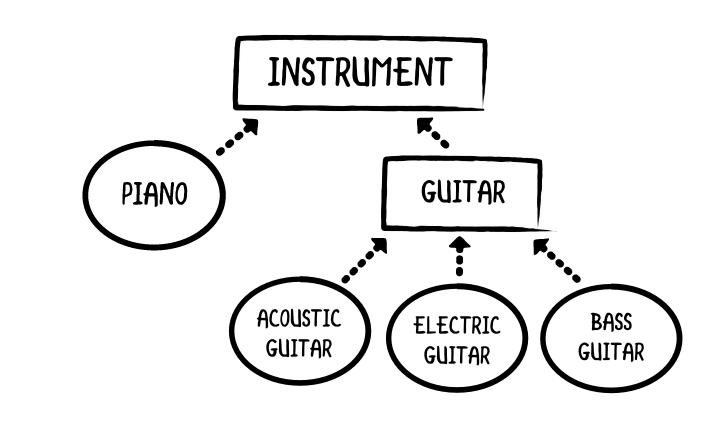
\includegraphics[scale=0.32]{oop-guitar-example.png}
\end{center}

\vspace{1cm}
\tiny{\flushleft{\href{https://www.raywenderlich.com/160728/object-oriented-programming-swift}{https://www.raywenderlich.com/160728/object-oriented-programming-swift}}}
}

%%%%%%%%%%%%%%%%%%%%%%%%%%%%%%%%%%%%%%%%%%%%%%%%%%%%%%%%%%%%%%%%%%%%%%%%%%%%%%%%
\frame{
\frametitle{A library to model functional annotation in Biology}
\begin{center}
  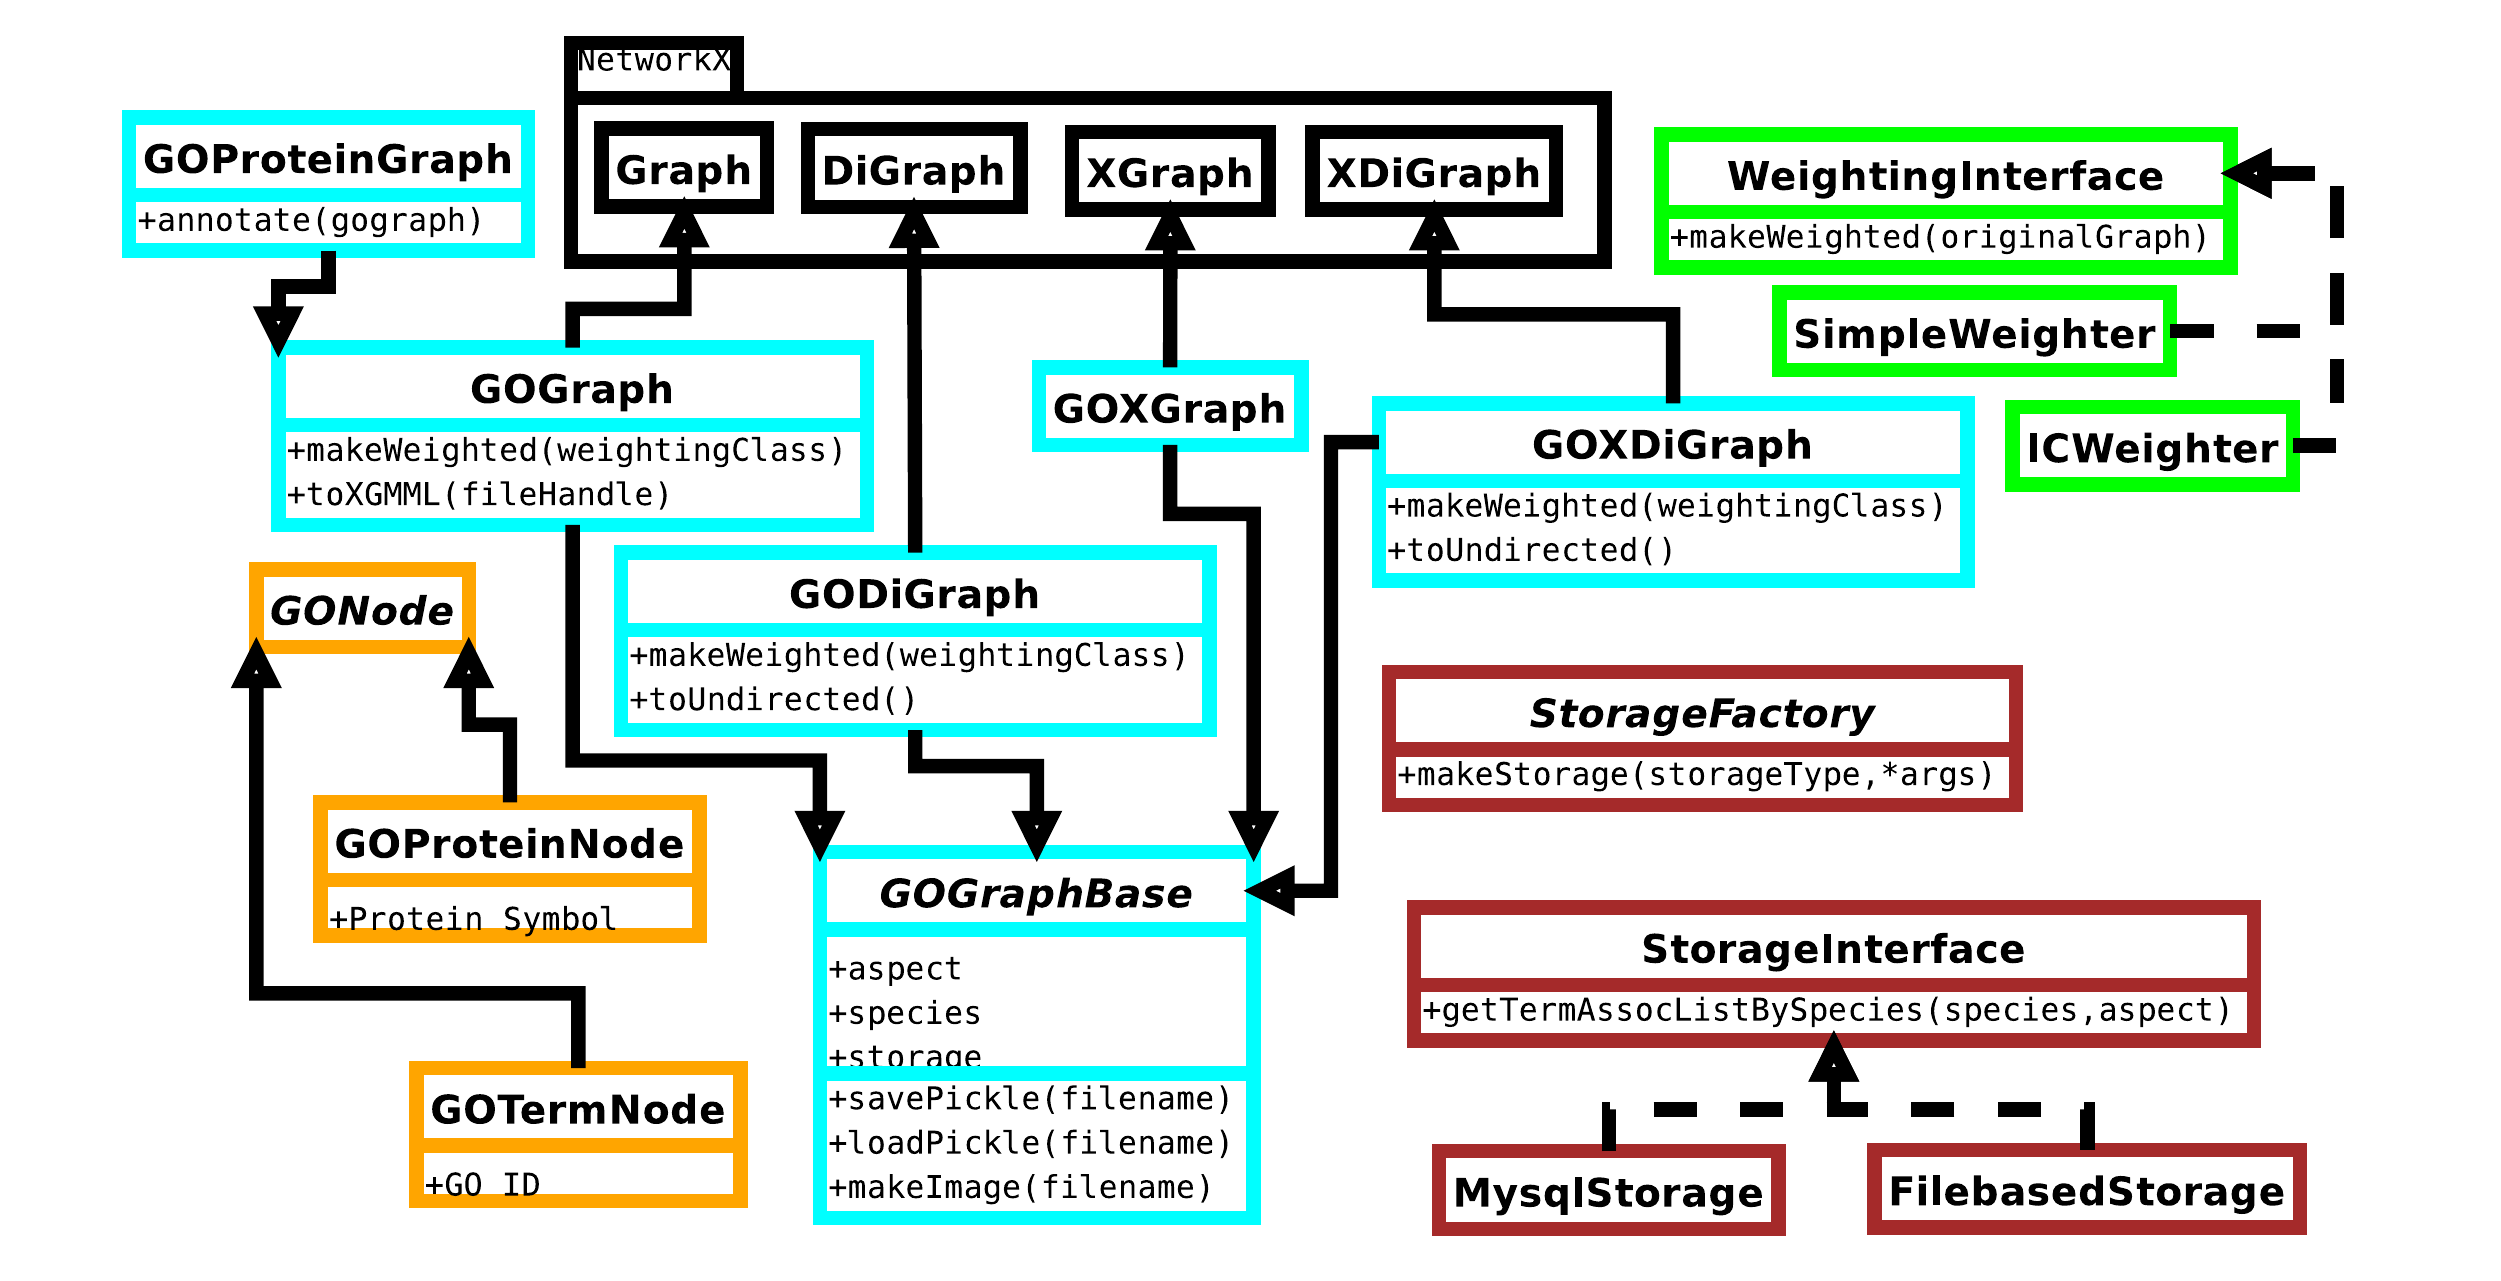
\includegraphics[scale=0.32]{muller-fig1.png}
\end{center}

This figure is a UML class diagram in which classes are grouped according to their functionalities....
\vspace{1cm}
\flushleft{\tiny{\href{https://bmcresnotes.biomedcentral.com/articles/10.1186/1756-0500-2-122}{https://bmcresnotes.biomedcentral.com/articles/10.1186/1756-0500-2-122}}}
}

%%%%%%%%%%%%%%%%%%%%%%%%%%%%%%%%%%%%%%%%%%%%%%%%%%%%%%%%%%%%%%%%%%%%%%%%%%%%%%%
\begin{frame}[fragile]
\scriptsize
\frametitle{You have been working with objects all along}
\begin{code}
print(type([1,2,3]))
<class 'list'>

print(type(1))
<class 'int'>

print(type(lambda x: x**2))
<class 'function'>
\end{code}

\begin{block}{}
 In Ipython or Jupyter \highlt{tab-completion} shows the methods and attributes, but with \texttt{dir} you can filter
\end{block}
\begin{code}
print([t for t in dir(np.array([1,2,3])) if 'set' in t.lower()])
['__setattr__', '__setitem__', '__setstate__', 'itemset', 'setfield', 'setflags']
\end{code}
\end{frame}


%%%%%%%%%%%%%%%%%%%%%%%%%%%%%%%%%%%%%%%%%%%%%%%%%%%%%%%%%%%%%%%%%%%%%%%%%%%%%%%%
\frame{
\begin{block}{}
A class is a blueprint that describes the format of an object.  How many classes?  How many objects?
\end{block}
\vspace{1cm}
\begin{center}
  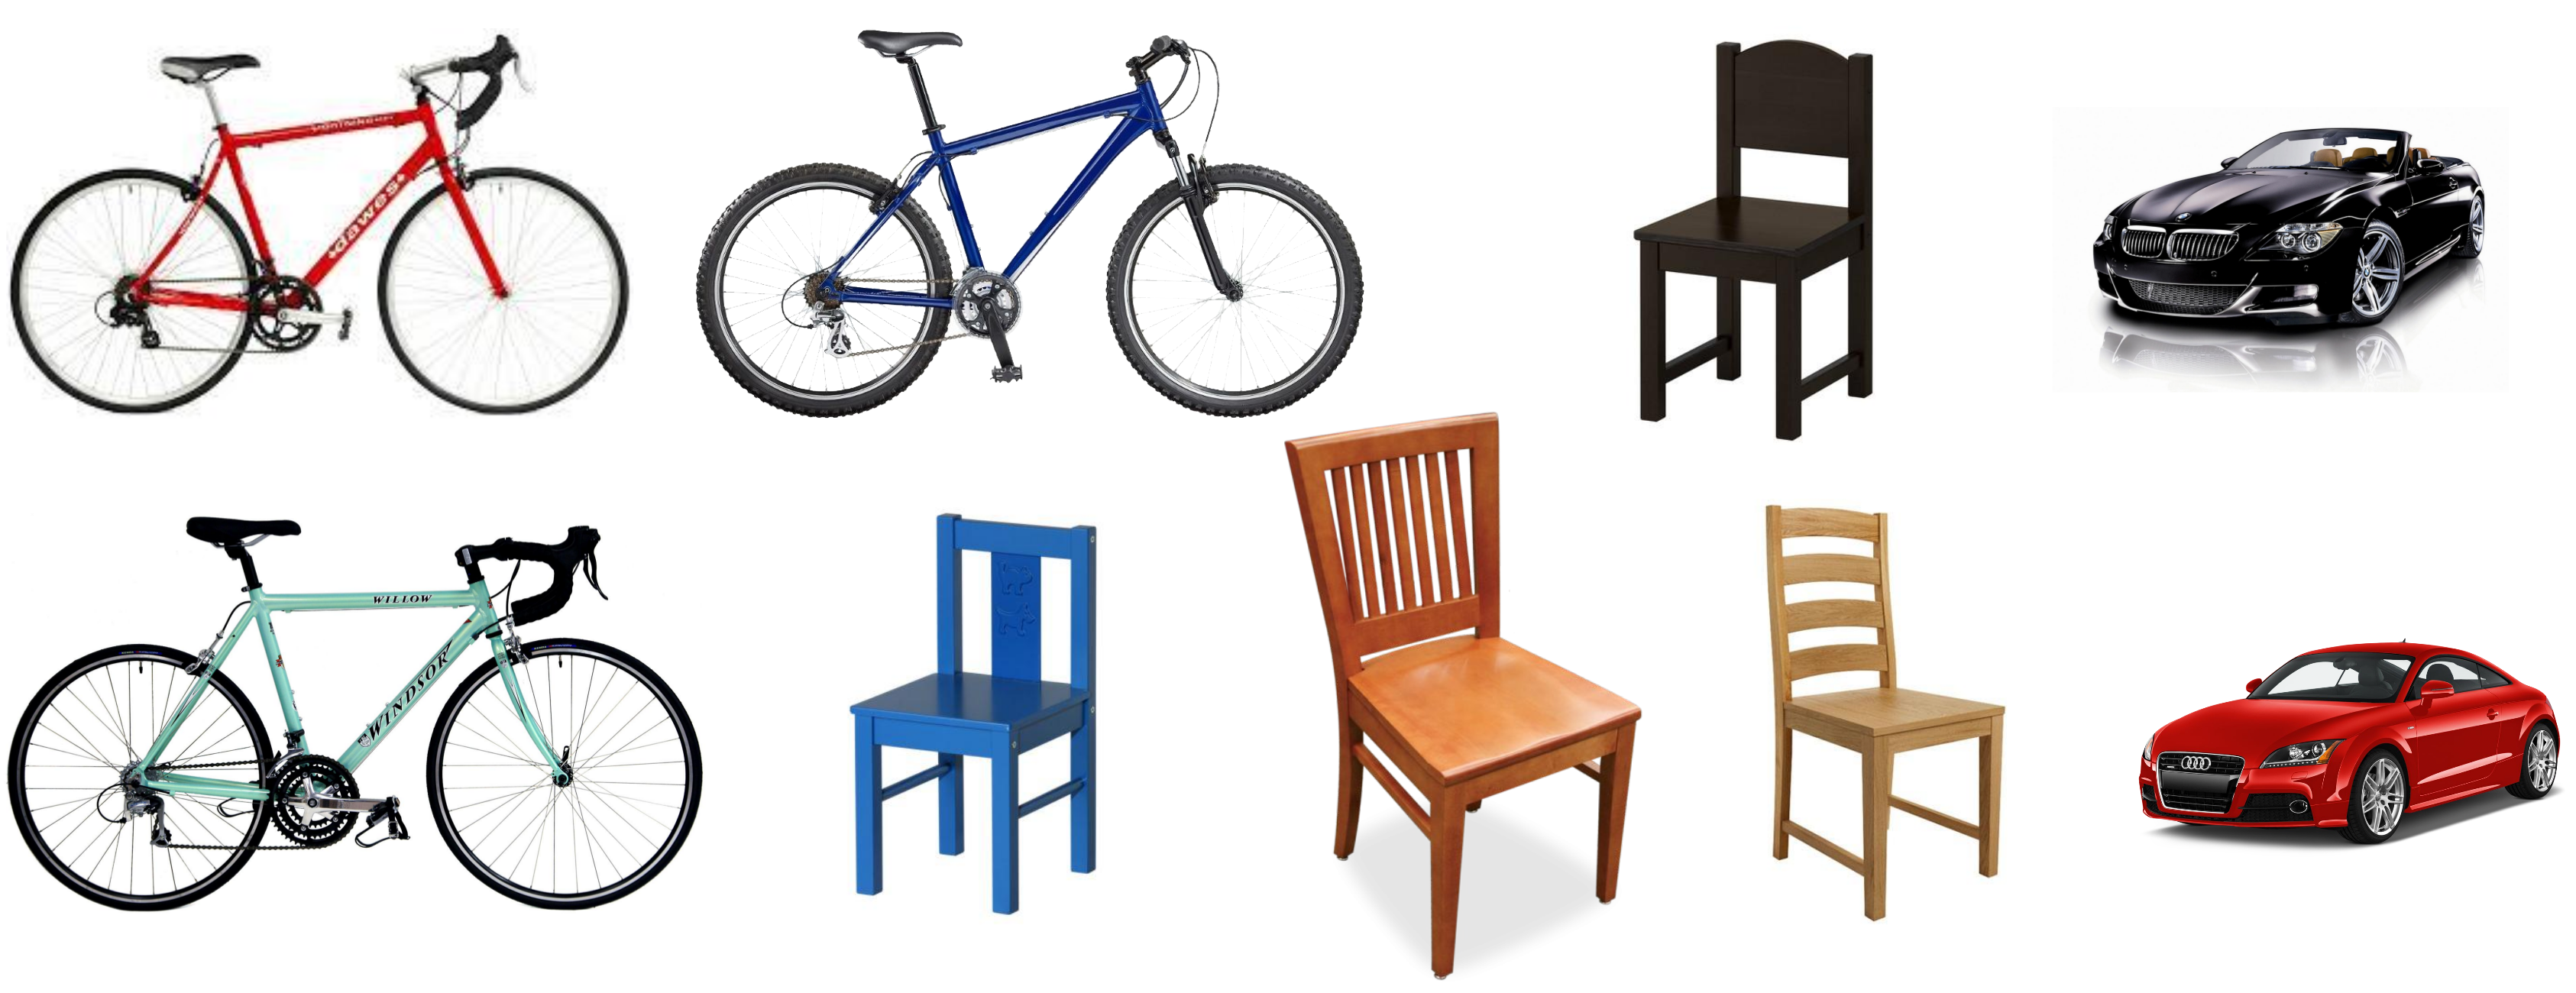
\includegraphics[scale=0.09]{how-many-classes.png}
\end{center}
}

%%%%%%%%%%%%%%%%%%%%%%%%%%%%%%%%%%%%%%%%%%%%%%%%%%%%%%%%%%%%%%%%%%%%%%%%%%%%%%%
\section{More Python}
\subsection{}
%%%%%%%%%%%%%%%%%%%%%%%%%%%%%%%%%%%%%%%%%%%%%%%%%%%%%%%%%%%%%%%%%%%%%%%%%%%%%%%

%%%%%%%%%%%%%%%%%%%%%%%%%%%%%%%%%%%%%%%%%%%%%%%%%%%%%%%%%%%%%%%%%%%%%%%%%%%%%%%
\begin{frame}[fragile]
\scriptsize

\frametitle{*args and **kwargs}
Convention and shorthand to refer to a variable number of arguments:
\begin{verbatim}

    For regular arguments, use *args:
        *args is a list
        def a_func(*args): takes multiple arguments
        Can also call function using a list

    For keyword arguments, use **kwargs:
        **kwargs is a dict
        def a_func(**kwargs): takes multiple keyword arguments
        Can also call function using a dict
\end{verbatim}
\end{frame}

%%%%%%%%%%%%%%%%%%%%%%%%%%%%%%%%%%%%%%%%%%%%%%%%%%%%%%%%%%%%%%%%%%%%%%%%%%%%%%%
\begin{frame}[fragile]

\begin{code}
def print_all(*args):
    for count,item in enumerate(args):
        print('{0}. {1}'.format(count, item))

print(print_all('earth','air','water','fire'))
\end{code}

\begin{codeout}
0. earth
1. air
2. water
3. fire
\end{codeout}
------------------------------------------------------------------------------------
\begin{code}
def list_all(**kwargs):
    for name, item in kwargs.items():
        print('{0} = {1}'.format(name, item))

list_all(blue_whale = 'Mammalia', lady_bug = 'Insecta')
\end{code}

\begin{codeout}
blue_whale = Mammalia
lady_bug = Insecta
\end{codeout}
\end{frame}

%%%%%%%%%%%%%%%%%%%%%%%%%%%%%%%%%%%%%%%%%%%%%%%%%%%%%%%%%%%%%%%%%%%%%%%%%%%%%%%%
\begin{frame}[fragile]
 
\frametitle{Magic Methods}
\footnotesize

Special methods, indicated by double underscore, that you can use to give
ubiquitous functionality of some operators to objects defined by your class.

\begin{table}
    \begin{tabular}{|c|l|}
    \hline
    Magic method                       & Purpose \\
    \hline
    \texttt{\_\_init\_\_(self, ...)}   & Constructor, initializes the class \\
    \texttt{\_\_repr\_\_(self)}        & Defines format for how object should be represented \\
    \texttt{\_\_len\_\_(self)}         & Returns number of elements in an object \\
    \texttt{\_\_gt\_\_(self, other)}   & Provides functionality for the $>$ operator \\
    \texttt{\_\_add\_\_(self, other)}  & Provides functionality for the $+$ operator \\
    \texttt{\_\_iadd\_\_(self, other)} & Provides functionality for the $+=$ operator \\ 
    \hline
    \end{tabular}
\end{table}
\vspace{1cm}
\begin{flushleft}
 \tiny \href{https://www.python-course.eu/python3\_magic\_methods.php}{https://www.python-course.eu/python3\_magic\_methods.php}
\end{flushleft}
\end{frame}

%%%%%%%%%%%%%%%%%%%%%%%%%%%%%%%%%%%%%%%%%%%%%%%%%%%%%%%%%%%%%%%%%%%%%%%%%%%%%%%
\frame{   
\frametitle{Morning Breakout}
\footnotesize
\begin{block}{Write a class to make an n-sided die}
After a die is instantiated let the user be able to query:
\begin{enumerate}
 \item How many sides it has
 \item What number is face up (its value)
\end{enumerate}

Also, let the user be able to:
\begin{enumerate}
 \item Roll the die
 \item Check compare the values of two die ($>, <, ==, \geq, \leq$)
\end{enumerate}
\end{block}
\begin{center}
  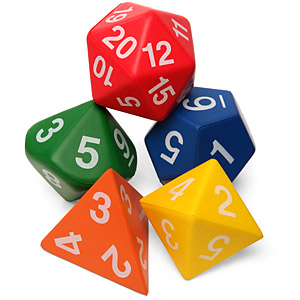
\includegraphics[scale=0.18]{gaming-dice.jpg}
\end{center}
You may use the \texttt{Simple.py} or the \texttt{Fruit.py} template.  Also, before you write any code \textbf{Write out the pseudocode}.
}

%%%%%%%%%%%%%%%%%%%%%%%%%%%%%%%%%%%%%%%%%%%%%%%%%%%%%%%%%%%%%%%%%%%%%%%%%%%%%%%
\frame{ 
\frametitle{Check-in questions}
\begin{block}{}
\highlt{Core questions}
\begin{enumerate}
 \item What is the difference between an object and a class?
 \item What is the difference between an attribute and a method?
 \item What is the role of \texttt{self} in defining a class?
 \item What can be used to give a custom class functionality similar to other classes?
 \item How can we see the attributes and methods available on an object?
\end{enumerate}
\end{block}
}

%%%%%%%%%%%%%%%%%%%%%%%%%%%%%%%%%%%%%%%%%%%%%%%%%%%%%%%%%%%%%%%%%%%%%%%%%%%%%%%
\section{Design}
\subsection{}
%%%%%%%%%%%%%%%%%%%%%%%%%%%%%%%%%%%%%%%%%%%%%%%%%%%%%%%%%%%%%%%%%%%%%%%%%%%%%%%

%%%%%%%%%%%%%%%%%%%%%%%%%%%%%%%%%%%%%%%%%%%%%%%%%%%%%%%%%%%%%%%%%%%%%%%%%%%%%%%
\frame{   
\frametitle{Objectives}
\scriptsize
\begin{block}{Morning}
 \begin{itemize}
  \item[\checkmark] Compare and contrast functional and object oriented programming
  \item[\checkmark] Given the code for a python class be able to: instantiate, call methods and access the attributes
  \item[\checkmark] Write the python code for a simple class
  \item[\checkmark] Design a program or algorithm in object oriented fashion
  \item[\checkmark] Be able to implement several \keywd{magic methods}
  \end{itemize}
\end{block}
  
\begin{block}{Afternoon}
 \begin{itemize}
  \item Intro to design patterns -- thinking in an object oriented fashion
  \item Intro to functional programming -- be able to compare and contrast functional and object oriented programming
  \item Intro to workflows
  \end{itemize}
\end{block}
}


%%%%%%%%%%%%%%%%%%%%%%%%%%%%%%%%%%%%%%%%%%%%%%%%%%%%%%%%%%%%%%%%%%%%%%%%%%%%%%%
\frame{ 
\frametitle{Functions, classes, modules and packages}
\scriptsize
\begin{itemize}
 \item \keywd{function} - A block of organized, reusable code that is used to perform a single related action 
 \item \keywd{class} - A template of reusable code that creates objects containing attributes and methods
 \item \keywd{module} - A file containing Python definitions and statements (e.g \texttt{mylib.py})
 \item \keywd{package} - Packages are a way of structuring Python’s module namespace
 \item \highlt{library} - A generic term for code designed to be usable by many applications
 \item \highlt{script} - a executable module
\end{itemize}
\begin{center}
------------------------------------------------------------------------------------
\end{center}

\begin{itemize}
 \item All packages are modules, but not all modules are packages 
 \item Any module that contains a \texttt{\_\_path\_\_} attribute is considered a package.  
 \item Packages may be installable via \texttt{run.py} and registered in PyPI 
\end{itemize}
 
The \href{https://pypi.python.org/pypi}{Python Package index} is where many packages live,
}

%%%%%%%%%%%%%%%%%%%%%%%%%%%%%%%%%%%%%%%%%%%%%%%%%%%%%%%%%%%%%%%%%%%%%%%%%%%%%%%
\begin{frame}[fragile]
 \frametitle{OOP design}

Build classes via:
\begin{itemize}
    \item Composition/aggregation:
        \begin{itemize}
            \item Class contains an object of another class with the desired functionality
            \item Often, just basic types: \texttt{str}, \texttt{float}, \texttt{list}, \texttt{dict}, etc.
            \item \textit{HasA} $\Rightarrow$ use members, aggregation
        \end{itemize}

  \item Inheritance
        \begin{itemize}
            \item Class specializes behavior of a base class
            \item \textit{IsA} $\Rightarrow$ use inheritance
            \item In some cases, derived class uses  a \textit{mix-in} base class only to provide functionality, not polymorphism
        \end{itemize}
\end{itemize}
\end{frame}
    
%%%%%%%%%%%%%%%%%%%%%%%%%%%%%%%%%%%%%%%%%%%%%%%%%%%%%%%%%%%%%%%%%%%%%%%%%%%%%%%
\begin{frame}[fragile]
 \frametitle{Interfaces}

\begin{block}{} 
 An interface is a contract between the client and the service provider:
\end{block}

\begin{itemize}
    \item Isolates client from details of implementation
    \item Client must satisfy preconditions to call method/function
    \item  Respect boundary of interface:
\end{itemize}

\begin{itemize}
    \item Library/module provides a service
    \item Clients only access resource/service via library
    \item Then bugs arise from arise incorrect access or defect in library
\end{itemize}
\end{frame}

%%%%%%%%%%%%%%%%%%%%%%%%%%%%%%%%%%%%%%%%%%%%%%%%%%%%%%%%%%%%%%%%%%%%%%%%%%%%%%%
\begin{frame}[fragile]
\frametitle{Test Driven Development (TDD)}
\footnotesize
Make sure your interface is intuitive and friction-free:

\begin{itemize}
    \item Use unit tests or specification test
        \begin{itemize}
        \footnotesize
            \item To verify interface is good before implementation
            \item To exercise individual functions or objects before application is complete
            \item Framework can setup and tear-down necessary test fixture
        \end{itemize}
    \item Stub out methods using pass
    \item Test Driven Development (TDD):
        \begin{itemize}
        \footnotesize
        \item Red/Green/refactor
        \item[1] Write unit tests
        \item[2] Verify that they fail (red)
        \item[3] Implement code (green)
        \item[4] Refactor code (green)
        \end{itemize}
    \item Use a \keywd{unit test} framework -- unittest (best), doctest, or nose
\end{itemize}
\begin{flushleft}
 \tiny \href{http://www.amazon.com/Verification-Validation-Scientific-Computing-Oberkampf/dp/0521113601/ref=pd_sim_14_2?ie=UTF8&refRID=1WP5FV5JCHXYAJAN6XAK}{Verification and Validation in Scientific Computing} discusses rigorous framework to ensure correctness
\end{flushleft}
\end{frame}

%%%%%%%%%%%%%%%%%%%%%%%%%%%%%%%%%%%%%%%%%%%%%%%%%%%%%%%%%%%%%%%%%%%%%%%%%%%%%%%
\frame{   
\frametitle{Afternoon Breakout}
\footnotesize
\begin{block}{Write a unit test to test for object equality}

\begin{enumerate}
 \item \texttt{run-tests.py} - controls all tests
 \item \texttt{unittests} - is a folder were the test scripts live
 \item \texttt{unittests/\_\_init\_\_.py} - controls what is run by \texttt{run-tests.py}
 \item \texttt{unittests/DieTest.py} - contains the actual tests for the Dice class
 \end{enumerate}

\begin{enumerate}
 \item Fill in the \texttt{testEquality} function
 \item Using the red/green/refactor procedure to write a new test for the \texttt{\_\_lt\_\_} magic method in \texttt{BaseDie}
\end{enumerate}
\end{block}

In part II, Just test something simple---exposure to this framework is what is important not the \highlt{coverage}

}

% %%%%%%%%%%%%%%%%%%%%%%%%%%%%%%%%%%%%%%%%%%%%%%%%%%%%%%%%%%%%%%%%%%%%%%%%%%%%%%%
% \begin{frame}[fragile]
% \footnotesize
% \frametitle{Unit tests}
% Verifying your code is correct, and finding and fixing bugs are critical skills:
% 
% \begin{itemize}
%  \item Just because your code runs, doesn't mean it is correct
%  \item Write unit tests to exercise your code:
%  
%  \begin{itemize}
%  \footnotesize
%   \item Ensures interfaces satisfy their contracts
%   \item Exercise key paths through code as well as corner cases
%   \item Identify any bugs introduced by future changes which break existing code
%   \item Test code before implementing entire program
%  \end{itemize}
% 
%  \item When unit tests fail, use a debugger to examine how code executes
%  \item Both are critical skills and will save you hours of time
%  end{itemize}
% \end{frame}

%%%%%%%%%%%%%%%%%%%%%%%%%%%%%%%%%%%%%%%%%%%%%%%%%%%%%%%%%%%%%%%%%%%%%%%%%%%%%%%
\begin{frame}[fragile]
\frametitle{Design Patterns}
\scriptsize
Many design patterns exist to standardize best practice and  they are worth learning if you regularly develop software
\vspace{0.5cm}

\begin{block}{Examples}
\begin{itemize}
 \item \highlt{MVC} (Separate out Model, View, Controller)
 \item \highlt{Abstract Factory} - Provide an interface for creating families of related or dependent objects without
specifying their concrete classes
 \item \highlt{Decorator} - Attach additional responsibilities to an object dynamically. Decorators provide a
flexible alternative to subclassing for extending functionality
 \item \highlt{Observer} - Define a one-to-many dependency between objects so that when one object
changes state, all its dependents are notified and updated automatically
 \item \highlt{Builder} - Separate the construction of a complex object from its representation so that the
same construction process can create different representations
\end{itemize}
\end{block}

\vspace{0.5cm}
Check out the book: \\
\textsl{Design Patterns: Elements of reusable Object-Oriented Software}
\end{frame}

%%%%%%%%%%%%%%%%%%%%%%%%%%%%%%%%%%%%%%%%%%%%%%%%%%%%%%%%%%%%%%%%%%%%%%%%%%%%%%%
\begin{frame}[fragile]
\frametitle{Design Patterns}
\footnotesize
\begin{center}
  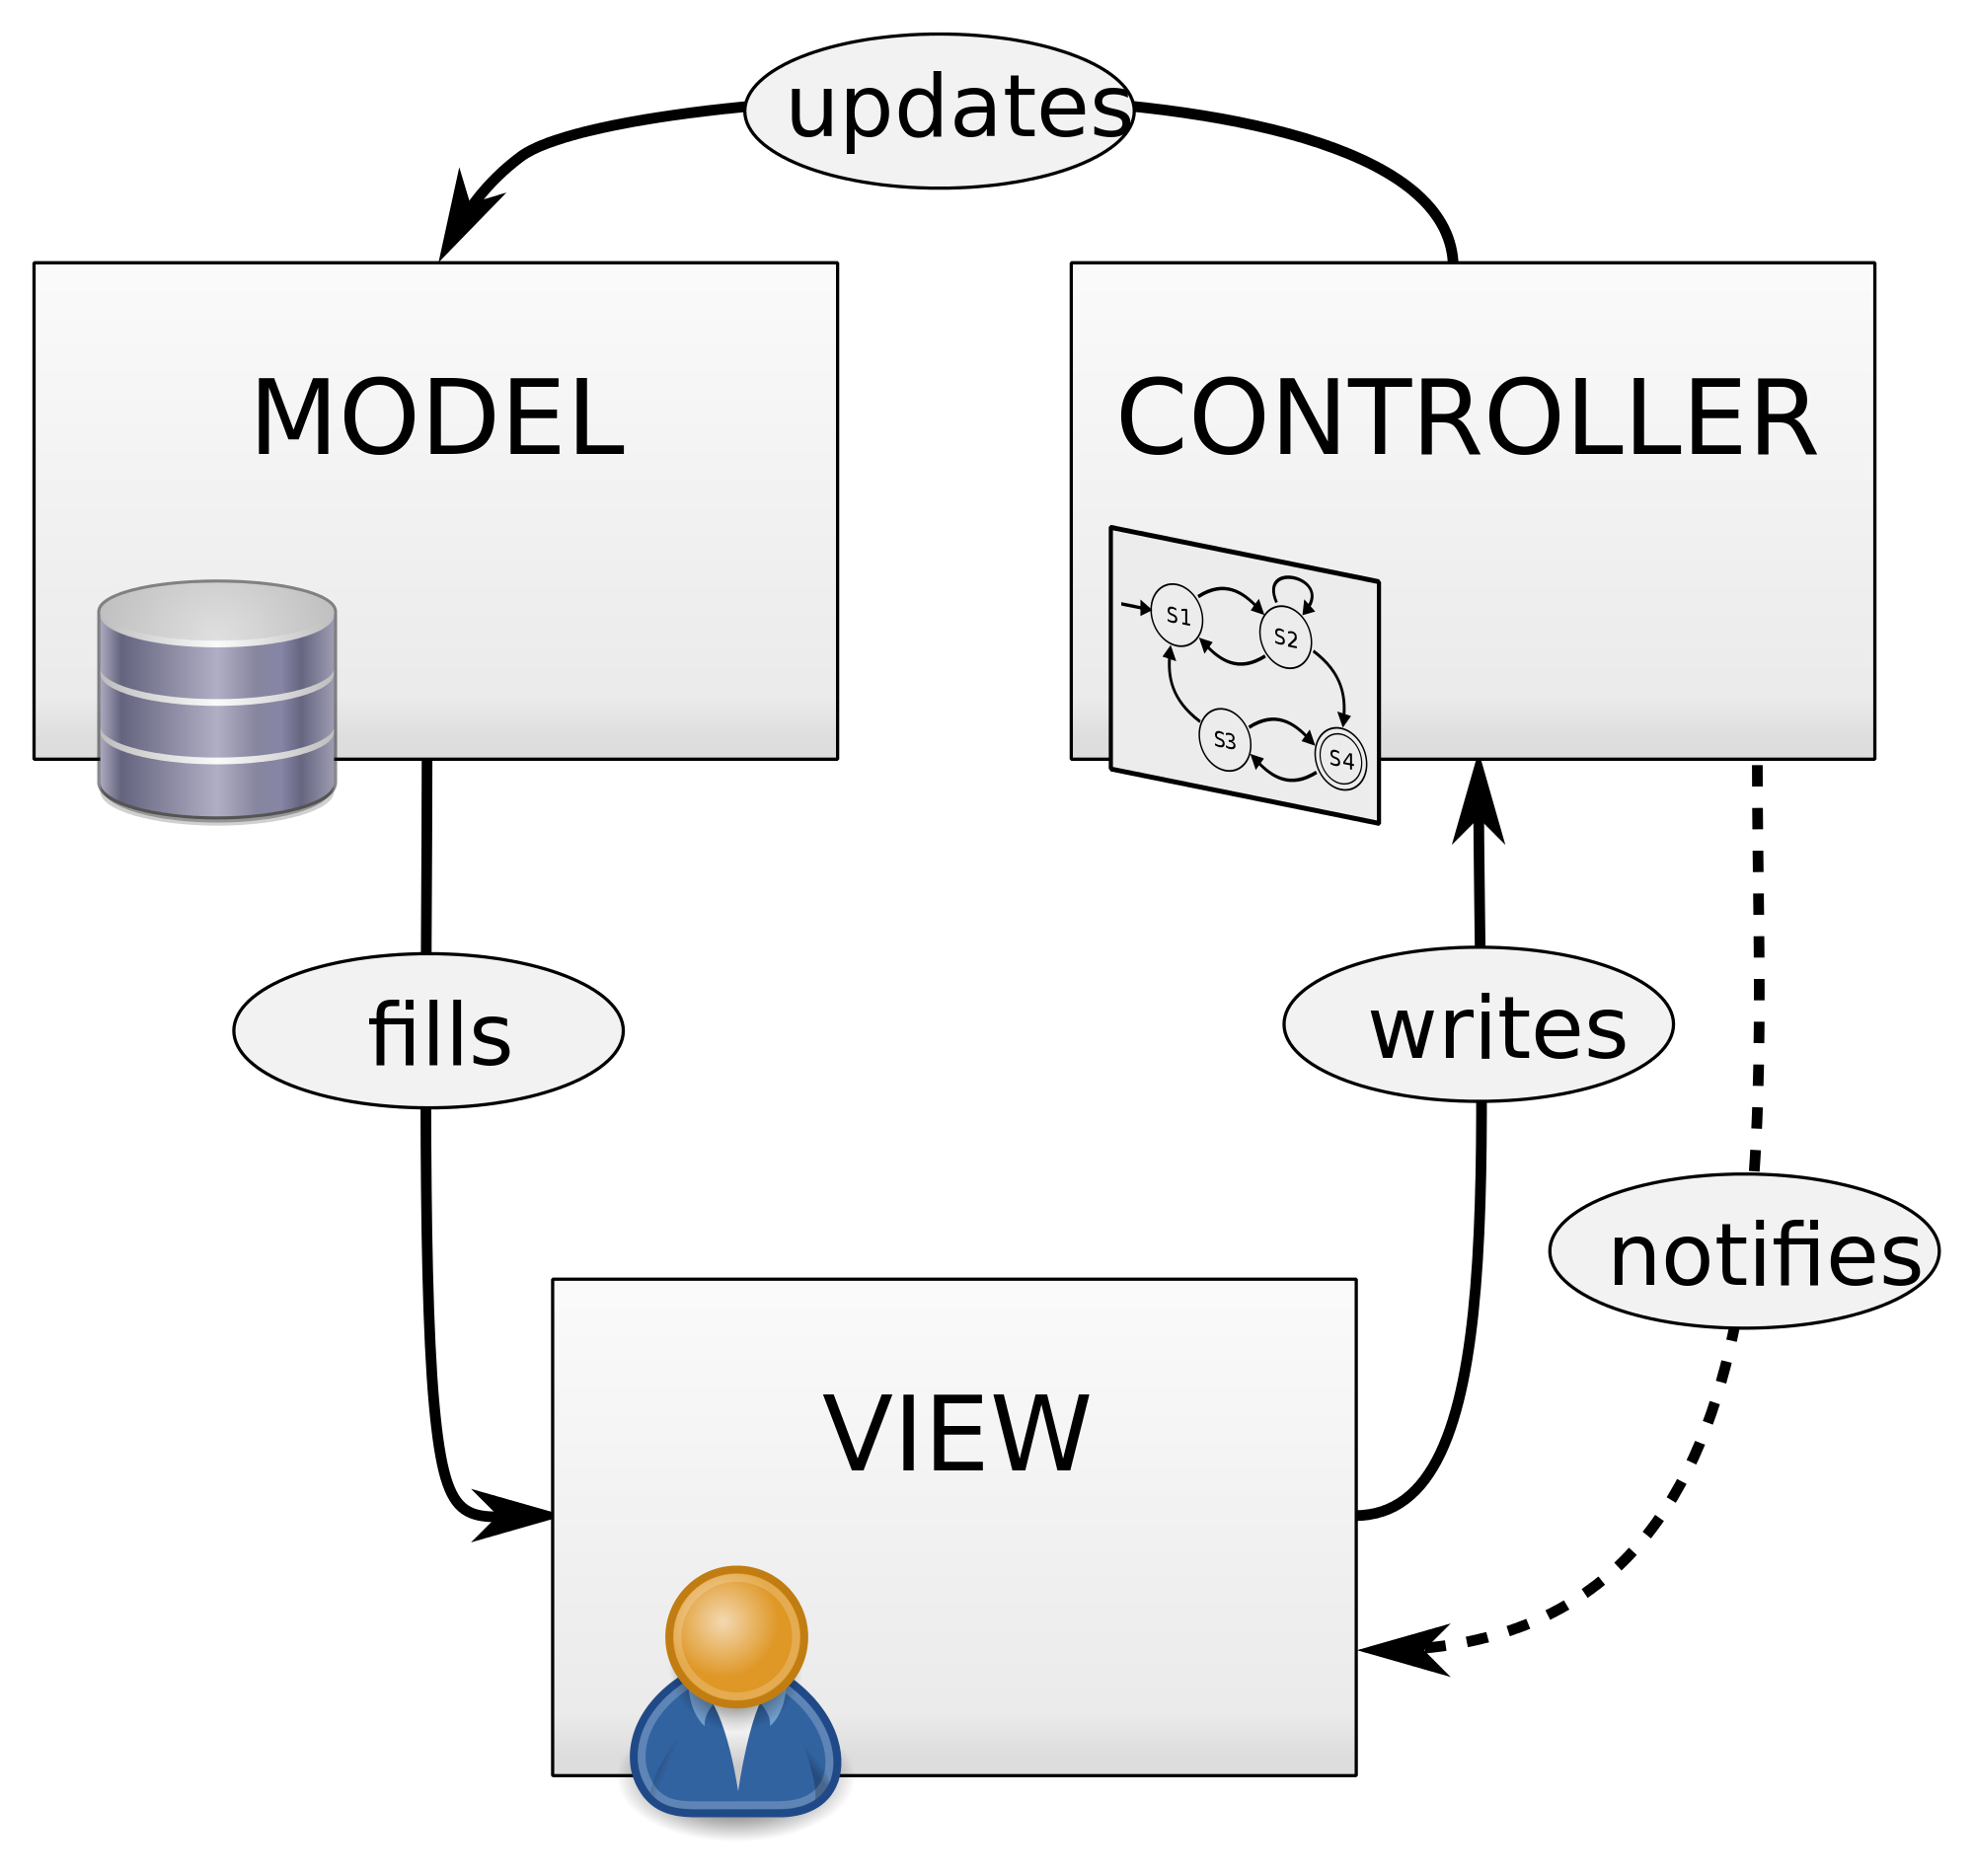
\includegraphics[scale=0.09]{mvc.png}
\end{center}
\begin{flushleft}
\tiny \href{https://commons.wikimedia.org/wiki/File:MVC\_Diagram\_(Model-View-Controller).svg}{https://commons.wikimedia.org/wiki/File:MVC\_Diagram\_(Model-View-Controller).svg}
\end{flushleft}
\end{frame}

%%%%%%%%%%%%%%%%%%%%%%%%%%%%%%%%%%%%%%%%%%%%%%%%%%%%%%%%%%%%%%%%%%%%%%%%%%%%%%%
\frame{ 
\frametitle{Check-in questions}
\begin{block}{}
\highlt{Core questions}
\begin{enumerate}
 \item How do we know if we need functions, modules, or packages? 
 \item What are the three key components of OOP? How do they lead to better code?
 \item How should I implement my code if the relationship is \textsl{Is A}? What if the relationship is \textsl{Has A}?
 \item What should you do ensure an object is initialized correctly?
 \item What are the benefits of TDD? What does Red/Green/Refactor mean?
\end{enumerate}
\end{block}
}

% %%%%%%%%%%%%%%%%%%%%%%%%%%%%%%%%%%%%%%%%%%%%%%%%%%%%%%%%%%%%%%%%%%%%%%%%%%%%%%
% \frame[allowframebreaks]{  
% \frametitle{References}
% \begin{tiny} \bibliography{pp.bib}
% \bibliographystyle{apalike}         % Style BST file
% \end{tiny}
% }

\end{document}